\documentclass[a4paper]{article}

%% Language and font encodings
\usepackage[english]{babel}
\usepackage[utf8x]{inputenc}
\usepackage[T1]{fontenc}
\usepackage{blindtext}
\usepackage{enumitem}
\usepackage{float}
\usepackage{commath}

%% Sets page size and margins
\usepackage[a4paper,top=3cm,bottom=2cm,left=3cm,right=3cm,marginparwidth=1.75cm]{geometry}

%% Useful packages
\usepackage{amsmath}
\usepackage{graphicx}
\usepackage[colorinlistoftodos]{todonotes}
\usepackage[colorlinks=true, allcolors=blue]{hyperref}

\newcommand{\ExternalLink}{%
    \tikz[x=1.2ex, y=1.2ex, baseline=-0.05ex]{% 
        \begin{scope}[x=1ex, y=1ex]
            \clip (-0.1,-0.1) 
                --++ (-0, 1.2) 
                --++ (0.6, 0) 
                --++ (0, -0.6) 
                --++ (0.6, 0) 
                --++ (0, -1);
            \path[draw, 
                line width = 0.5, 
                rounded corners=0.5] 
                (0,0) rectangle (1,1);
        \end{scope}
        \path[draw, line width = 0.5] (0.5, 0.5) 
            -- (1, 1);
        \path[draw, line width = 0.5] (0.6, 1) 
            -- (1, 1) -- (1, 0.6);
        }
    }



\pagestyle{headings}
\begin{document}
\begin{titlepage}

\centering

\hrulefill\par
\vspace{1cm}
{\scshape\LARGE University of Saint Etienne\par}
\vspace{1cm}
{\scshape\Large Deep Learning \par}
\vspace{1cm}
{\huge\bfseries Project rapport -- Detection of plant pathology with Deep Learning \par}
\vspace{1cm}
{\Large\itshape BADIKIAN Guillaume, CLEMENT Gauthier, LOEW Benoît, REVOUY Théo, SANOU Abou\par}
\vspace{0.8cm}
{\large the \today\par}
\vfill
\underline{Teacher :} \par
HABRARD \textsc{Amaury} \par
\hrulefill\par

\end{titlepage}
\tableofcontents




\newpage

\section{Context of study: }

Failure to identify the many diseases affecting agricultural crops will contribute to the misuse of chemicals, contributing to the emergence of resistant strains of pathogens, higher input prices, and more epidemics with severe economic losses and environmental impacts. Current human screening-based diagnosis of disease is time-consuming and expensive, and while computer vision-based models are efficiently promising, the high variability of symptoms due to the age of infected tissues, genetic differences and light conditions in trees reduces the precision of detection.

\section{Protocol : }
In this part, we are going to explain how we will proceed to reach the goal of this project.
In order to perform with all details around this study, firstly we will figure out the state-of-art of deep learning applied to image classification.
Secondly, we will talk about our task which is plant pathology classification by summarising the previous studies on this field.
By the end of this report, we will propose our model, its parameters and the paradigm of training that we will use in order to optimize the model.  


\section{State-of-art: }
\subsection{Computer Vision}
Computer vision is an interdisciplinary scientific field that provides answers on how a computer can acquire knowledge from images and videos. 
From an engineering perspective, it seeks to understand and automate the tasks that the human visual system can perform \cite{vision}.
Computer vision tries to bring solutions to problems related to the automation of certain visual tasks. These include[4]  :

\subsubsection{Image Classification: }
Image classification involves a variety of challenges, including point of view variation, scale variation, intra-class variation, image distortion, image occlusion, lighting conditions, and background clutter.
Commonly the data-driven approach is used to choose the right model in order to do the best classification accuracy.
Basically the Convolutional Neural Networks (CNNs) is the most famous architecture used for image classification.

\subsubsection{Object Detection:}
Object detection is different from the Classification Task but uses it to achieve his goal. The aim of this task is firstly to identify objects in an image or a video and then to classify each object in order to produce a list of object categories present in the image along with an axis-aligned bounding box indicating the position and scale of every instance of each object category.

\subsubsection{Object Tracking :}

The aim of this is to track objects generally in the frame of a video. It is used basically in real-time context. This exploit is the sum of many techniques: Firstly in each frame, we have to identify the objects and then to classify them in one class. At the end, it makes a relation between the object in successive frames in order to track the object over the time.  

\subsubsection{Semantic Segmentation :}
The aim of Semantic Segmentation is to be able to make semantic division into image. More specifically, the goal of semantic image segmentation is to label each pixel of an image with a corresponding class of what is being represented. Because we're predicting for every pixel in the image, this task is commonly referred to as dense prediction.

\subsection{Solution for computer vision: }
Computer vision solutions are on the rise. Every year new techniques and models are introduced. In order to understand this field it's essential to know the basics and the genesis of it.
First of all, machine learning techniques did their introduction in the computer vision field with the geometric techniques such as Delaunay and Voronoï meshes \cite{fondationvision} used to perform computer vision tasks. These techniques were not robust and precise enough for concrete applications.
In the light of the fast development of machine learning techniques and the processing capacity of computers, the idea of using these techniques on images has emerged.
Now let’s talk about machine learning techniques for computer science. In fact, the kind of models adapted to Computer vision comes from the subfield of Machine learning which is Deep Learning.

%\subsubsection{Relevant solution of Deep Learning for Computer Vision :}
Deep learning proposes many techniques or models based on the artificial neural network and a lot of relevant models for Computer Vision. However most of them have been based on the Convolution Neural Network.
So before diving deep into these different models, let's bring some explaining on CNN.
The convolution neural network is very similar to the basic neural network but very special thanks to its capacity for processing data with a grid such as topology do. 
In addition, the CNN with sparse interaction between layers decreased drastically the numbers of the parameters of the neural network. It is also based on Equi-variant Representation.  

This network consists of multiple layers and we will have to learn the weights and biases.
Let's note that there is a last fully connected layer and let's specify the main function or layer of the CNN.
Basically, in the convolution neural network, there are four kinds of layers : Convolution Layer, Pooling Layer, Activation layer and Fully-Connected layer. 
\begin{itemize}
    \item{\textbf{ Convolution Layer :} The Convolution layer is usually the first layer in CNN where we convolve the image or data using a filter or a kernel. Filter are small units that we apply across the data  through a sliding window (stride). The depth of the filter is the same as the input, so for a color image (depth 3) we will apply a filter of a depth 3. 
    To clarify this, we will compute the sum of elements from Hadamard product (also known as the element-wise, entrywise or Schur product) between the image window and the kernel.  }
    
    \begin{figure}[H]
      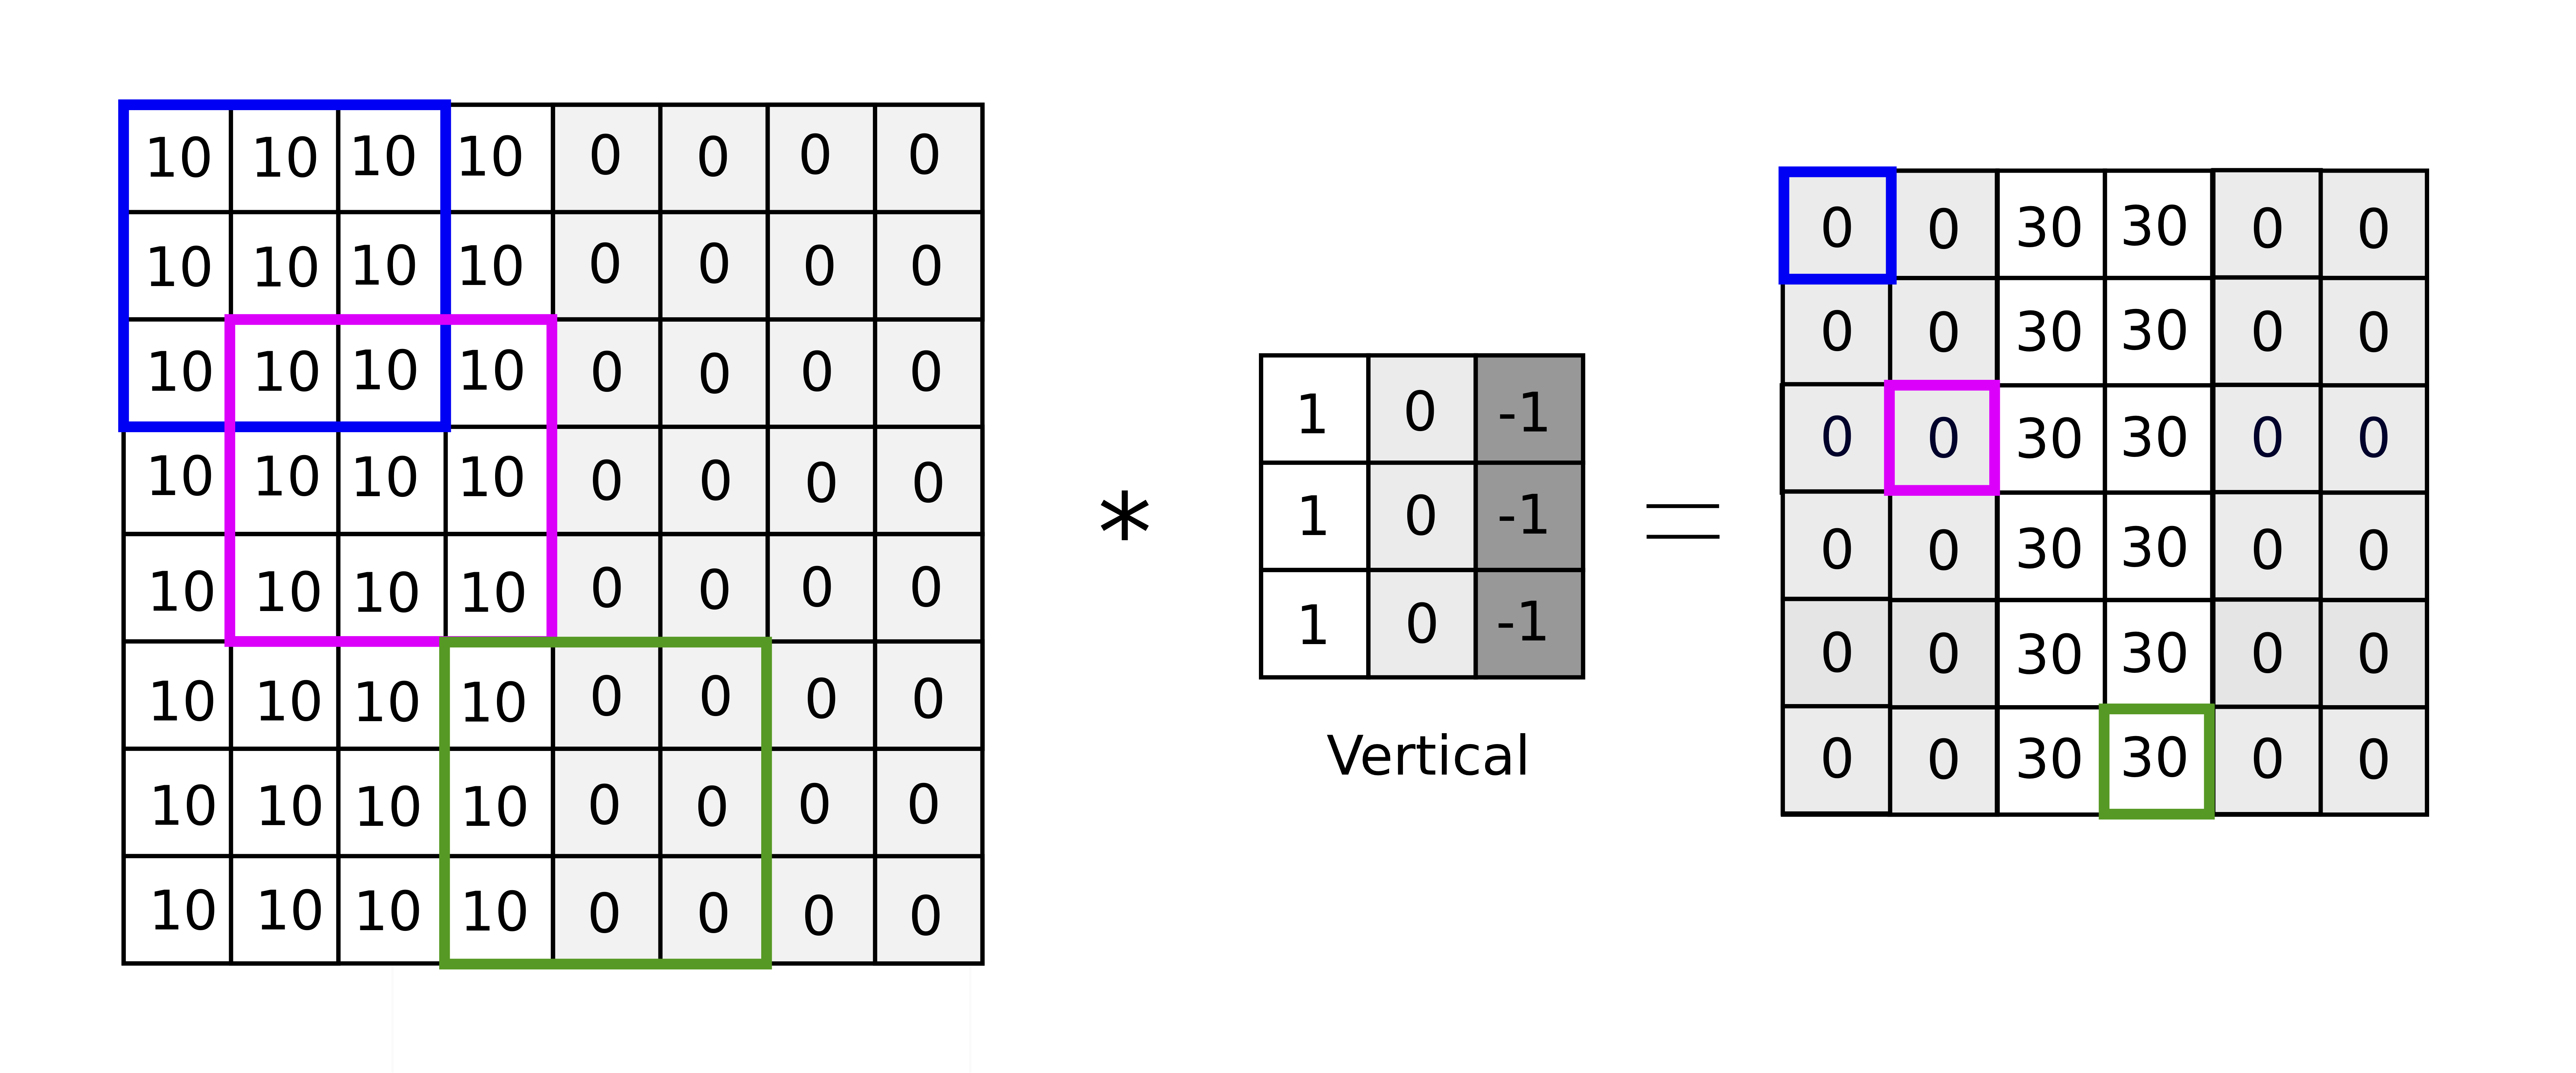
\includegraphics[width=\linewidth]{images/edge-detection-vertical.png}
      \caption{Convolution illustration: Image from \cite{cnnAnh}}
      \label{fig:boat1}
    \end{figure}
    
    \item{\textbf{Pooling Layer :} It is the most used layer in Convolution Neural Network. It is used in order to reduce the dimension of the matrix (Image in our case) in order to reduce the computation power required during the convolution operation.
        In the same way, pooling layers can reduce the overfitting risks of the model. Indeed, Image is a high dimensional data and we know that high dimensional data can cause the curse of dimensionality. It can bring up an Overfitting problem. So by avoiding it, we will reduce the chances of overfitting.
        Let's explain the operation of pooling with two hyper parameters. Dimension of spatial extent and the stride. 
        The stride is how many features the sliding window skips along the width and height, which is similar to what we saw in the convolution layer. Pooling operation will take a specific value to represent one zone of an image according to the kind of pooling used (Max, Min, Avg).
        For the following example in the schema, the dimension is 2*2 and the stride is 2.
}
  \begin{figure}[H]
      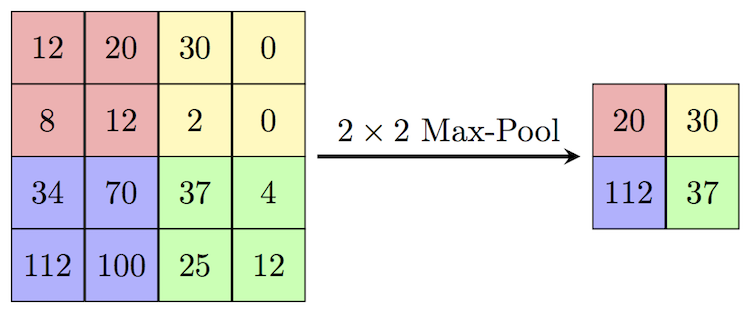
\includegraphics[width=\linewidth]{images/pooling.png}
      \caption{Max pooling illustration: Image from \cite{cs231n}}
      \label{fig:boat1}
    \end{figure}


    \item{\textbf{Activation Layer :}
    In a Convolution Neural Network or generally in Any Neural Network, we need a non-linear layer which consists of an  activation function that takes the feature map generated by the previous layer and creates the activation map as its output.
    The activation function is an element-wise operation over the input volume and so the dimensions of the input and the output are identical.\cite{nonlinear}
    The activation function is the function embedded in each of the neurons. Its goal is to normalize the output of the neurons depending on the input.
    Our CNN models will be based on DNNs. %Thus, we need to take advantage of back-propagation by using non-linear activation functions.
    Let’s compare the following ones.
    \begin{itemize}
        \item{\textbf{Sigmoid :}  
        It’s the most known nonlinear function. It prevents output jumps and normalizes the output between 0 and 1. Nevertheless, it is known to have a gradient vanishing problem happening with high input values.
        }
        \item{\textbf{ReLU : (Rectified Linear Unit) : }
        This function is close to linear one but allows backpropagation. But a backpropagation problem happens when the input is close to zero or negative.
}
    \item{\textbf{Softmax :}
        This function is the only one of these three to handle multiple classes as input. Typically used to classify the outputs.
        }
        
    \end{itemize}

}

\item{\textbf{Fully Connected Layer :}
 After getting a feature map from the convolution operator, we will learn non-linear combinations of features. Essentially the convolution provides a meaningful, low-dimensional and invariant feature space. The fully-connected layer will learn a nonlinear function from this feature space obtained.
 But the output of the Convolution (Convolution + Pooling) is commonly a matrix although
 the Fully-Connected layer must receive a vector. In order to be able to pass the matrix as an input of a fully-connected layer, we will apply the flattened operation which transforms a matrix in a vector.
}
\end{itemize}



\section{Project Description : }
This project can be viewed as an image classification task in machine learning(Deep Learning).
There are 5 categories : four diseases and healthy leaves.
Our goal is to classify in an accurate way the image of the leaves in one or multiple categories of diseases. Indeed one leave can have multiple diseases and  our model must be able to detect this kind of situation.\\	
\textbf{Image Classification} is a fundamental task. The goal is to classify the image by assigning it to a specific label. Typically, Image Classification refers to images in which only one object appears and is analyzed. In contrast, object detection involves both classification and localization tasks, and is used to analyze more realistic cases in which multiple objects may exist in an image. \href{https://paperswithcode.com/task/image-classification}{(Image classification)\ExternalLink}
\newpage

\section{Data description or exploration: }
Before any formal analysis of the data, we have to know the number of items and the variables in the data set, the number of missing observations and the general assumptions the data suggest. To answer these questions, an initial exploration of the dataset will allows us to become familiar with the data that will handle.
Data exploration or data description is a very important phase in any machine learning project. This step allows us to get more details about the dataset which we will use to train our model.

For our project we got the dataset from kaggle: \href{https://www.kaggle.com/c/plant-pathology-2020-fgvc7}{Link\ExternalLink}. The database folder consists of \textbf{3642} images in \textbf{jpg} format. Each image is in \textbf{2048} pixels * \textbf{1365} pixels with \textbf{3} channels(RGB).
Added to these images, there are three others files.
\begin{itemize}
    \item sample\_submission.csv: this is the sample for the submission. We will start by simply looking at a few random samples.
    \item train.csv: this file contains the training set with its labels. We will use it during the training of the model.
    \item test.csv: this file will contains the test set.
\end{itemize}

After describing the files which constituted the dataset, we will explore it through statistical metrics.

Let's start with the distribution of the dataset row (image) over the classes. To sum up this information let's draw a pie chart ~\ref{fig:pie}


    \begin{figure}[H]
      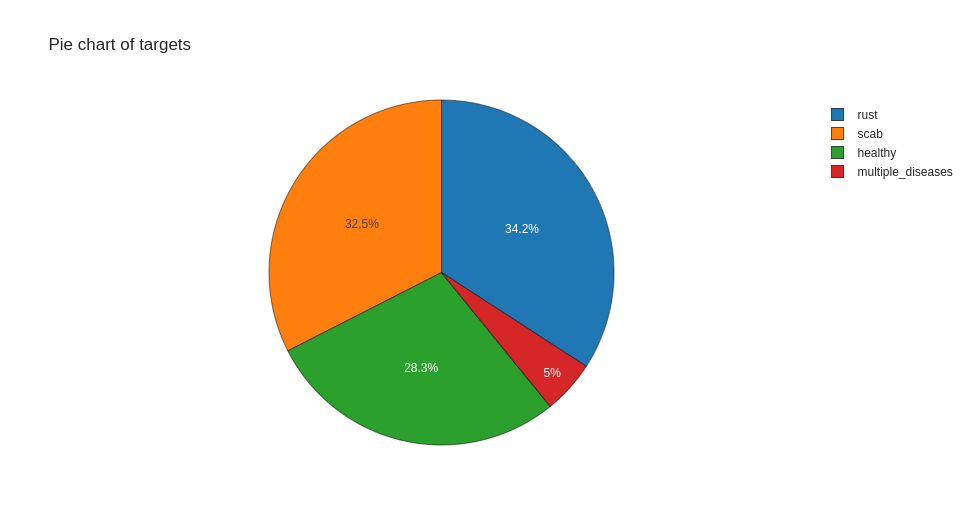
\includegraphics[width=\linewidth]{images/pie.png}
      \caption{Distribution of color: Image from "https://www.kaggle.com/c/plant-pathology-2020-fgvc7"}
      \label{fig:pie}
    \end{figure}


The amount of photos is quite similar for each target, unless for multiple diseases class. \\

   \begin{figure}[H]
      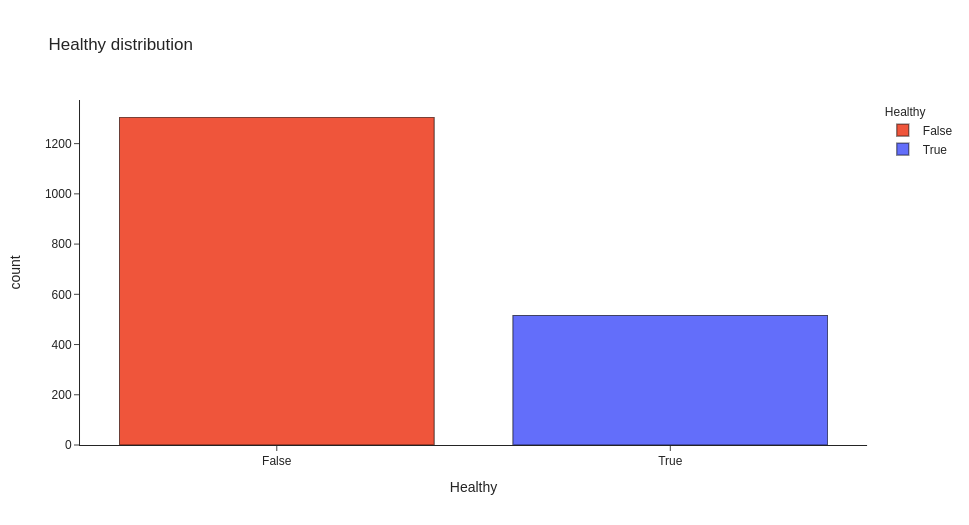
\includegraphics[width=\linewidth]{images/histo_classes.png}
      \caption{Distribution of image in: Diseases or Not from "https://www.kaggle.com/c/plant-pathology-2020-fgvc7"}
      \label{fig:histo}
    \end{figure}

Let's explore the color distribution of images refers to figure ~\ref{fig:boxplot}:
 
    \begin{figure}[H]
      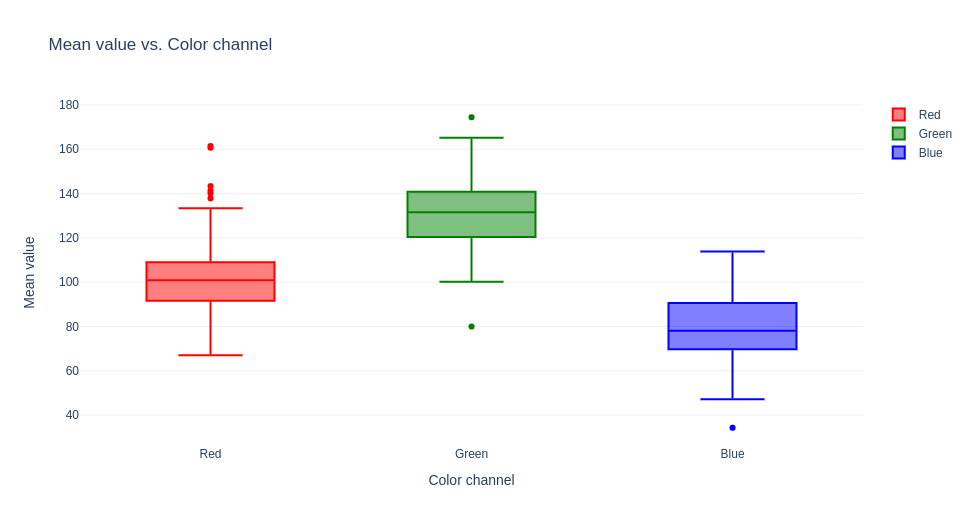
\includegraphics[width=\linewidth]{images/boxplot.png}
      \caption{Distribution of item in classes: Image from  "https://www.kaggle.com/c/plant-pathology-2020-fgvc7"}
      \label{fig:boxplot}
    \end{figure}

Now, let see the distribution on the histogram, confer figure :

  \begin{figure}[H]
      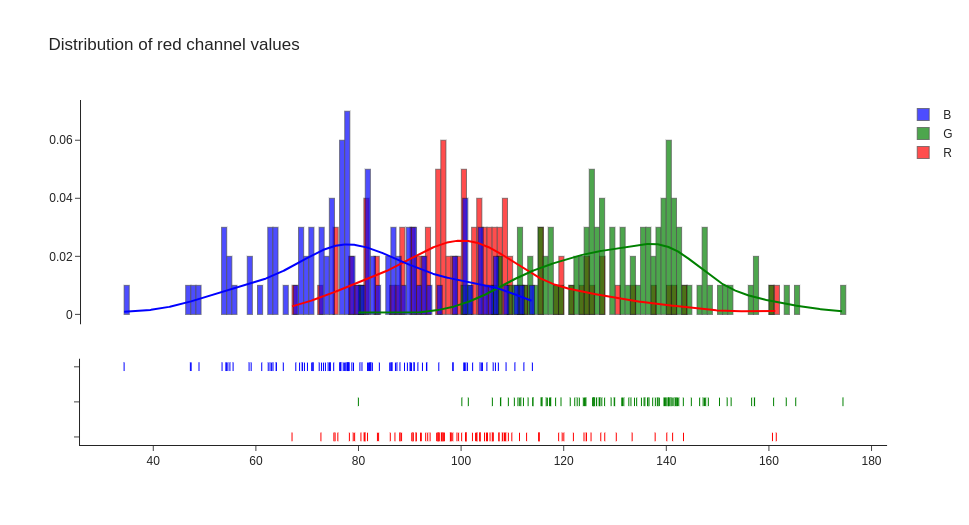
\includegraphics[width=\linewidth]{images/histo.png}
      \caption{Distribution of color: Image from "https://www.kaggle.com/c/plant-pathology-2020-fgvc7"}
      \label{fig:boxplot}
    \end{figure}

We can notice that the color distribution shape for each channel is quite similar with some shifts. Of course the green one is the most prominent. From this point, we can suppose that the model classifying process may rely on this distribution.


After the exploration of the data we will go on to the preparation of the data in order to make it easy for the extraction of knowledge on the model.


\section{Data preparation :}

%/ Data augmentation
Data augmentation is the concept aiming to slightly modify the original database in order to make it clean. A clean database allows a more exhaustive learning and prevents more overfitting. The different techniques used in data augmentation and preparation have to rely on the specific application needs. In the context of computer vision, we speak about image preparation. There are several techniques coming from the potential, pictures environment related, image distortion. These can be due to the diversity of devices leading to different processing of the the same captured picture. Weather conditions or the point of view that the photograph has chosen for his pictures can also influence the picture. The image preprocessing techniques aim to to simulate those diverging behaviours. \\

This is a crucial part for our study. Indeed, performing Image classification implies dealing with high dimensions data. So in order to facilitate the training of the data in this crucial context, we have to prepare images. We use the following process :
\subsection{Canny edge detection :}
Canny edge detection is an edge detection algorithm as noticed by its name. It was created by John F. Canny in 1986. The algorithm involves in several steps.
\begin{itemize}
    \item { \textbf{Noise reduction:} Since edge detection is susceptible to noise in an image, we remove the noise in the image using a 5x5 Gaussian filter\cite{guassian}. So recall the Gaussian function in one dimension also call function of density: 
     
 %    \begin{document}
\[
%\frac {1}{\sigma \sqrt{2\pi \sigma^2}}
P(x) = \frac{1}{{\sigma \sqrt {2\pi } }}e^{{{ - \left( {x - \mu } \right)^2 } \mathord{\left/ {\vphantom {{ - \left( {x - \mu } \right)^2 } {2\sigma ^2 }}} \right. \kern-\nulldelimiterspace} {2\sigma ^2 }}}
\]
%\end{document}
 Let's assume that sigma is the standard deviation of the distribution (in our case of image). The distribution is assumed to have a mean of 0. More simply  will reduce the range of the dataset around the mean 0; with the standard or (ecart-type) 1.
Let's notice that as well as standard deviation is large the range of the distribution will be large.

In our case we will use the gaussian function on two dimensions as following :
\[
%\frac {1}{\sigma \sqrt{2\pi \sigma^2}}
P(x,y) = \frac{1}{{\sigma \sqrt {2\pi } }}e^{{{ - \left( {x^2 + y^2} \right) } \mathord{\left/ {\vphantom {{ - \left( {x^2 + y^2} \right)^2 } {2\sigma ^2 }}} \right. \kern-\nulldelimiterspace} {2\sigma ^2 }}}
\]
Now let's see how we are going to apply this distribution on our dataset or more clearly how to bring back our distribution in normal distribution. 
Firstly we have to compute the standard deviation and mean of each dimension of distribution of the images. 
After that, for each value we can do the values minus the mean in order to get the mean of the distribution to 0. And we have to divide the result value with the standard of derivation in order to get the standard of derivation to 1. With these metrics we can define the Gaussian functions in the image field this function is a kernel or matrix. 
After getting a Gaussian kernel which is a matrix, we have to apply convolution operation between the kernel and each image or each channel of image.
}


\item{\textbf{Finding Intensity Gradient of the Image \cite{gradient}: } 
	First, the gradient in computer vision is the directional change in image if we loop on coordinate. Now we have to compute edge gradient and Angle of gradient.
    Let consider the image I represented in a matrix, the gradient in the pixel with the coordinates x=c and y=r can be compute as follows :
    \begin{equation}
    dx = I(c+1, r) - I(c-1,r) \\\
    dy = I(c,r+1) - I(c,r-1) 
    \end{equation}
    This means calculating the partial derivative of the function represented in our case by the matrix.
    I(x,y) is a luminosity in one channel 
    The gradient magnitude is how strong is the change of the luminosity if we can position it in image.
	To find the Intensity Gradient of the Image, we need two metric :
	The gradient orientation and the Edge Gradient.
	The gradient orientation is computed as followed :
	\begin{equation} 
	\theta = \tanh^{-1}{(dx^2 + dy^2)}
	\end{equation}
	The magnitude or edge gradient  equals :
	\begin{equation} 
	Magnitude = \sqrt{(dx^2 + dy^2)}
	\end{equation}
}

\item{\textbf{Rounding : } The gradient is always perpendicular to edges. So, it is rounded to one of the four angles representing vertical, horizontal and two diagonal directions.

\item {\textbf{Non-maximum suppression : } After getting the gradient magnitude and direction, a full scan of the image is done to remove any unwanted pixels which may not constitute the edge. For this, we check every pixel for being a local maximum in its neighborhood in the direction of the gradient.
}

\item{\textbf{Hysteresis Thresholding:} This stage decides which parts are edges and which are not. For this, we need two threshold values, minVal and maxVal. Any edges with intensity gradient greater than maxVal are considered edges and those lesser than minVal are considered non-edges, and discarded. Those who lie between these two thresholds are classified edges or non-edges based on their neighborhood. If they are near “sure-edge” pixels, they are considered edges, and otherwise, they are discarded.
}



}
\begin{figure}[H]
\centering
\begin{subfigure}{\textwidth}
  \centering
  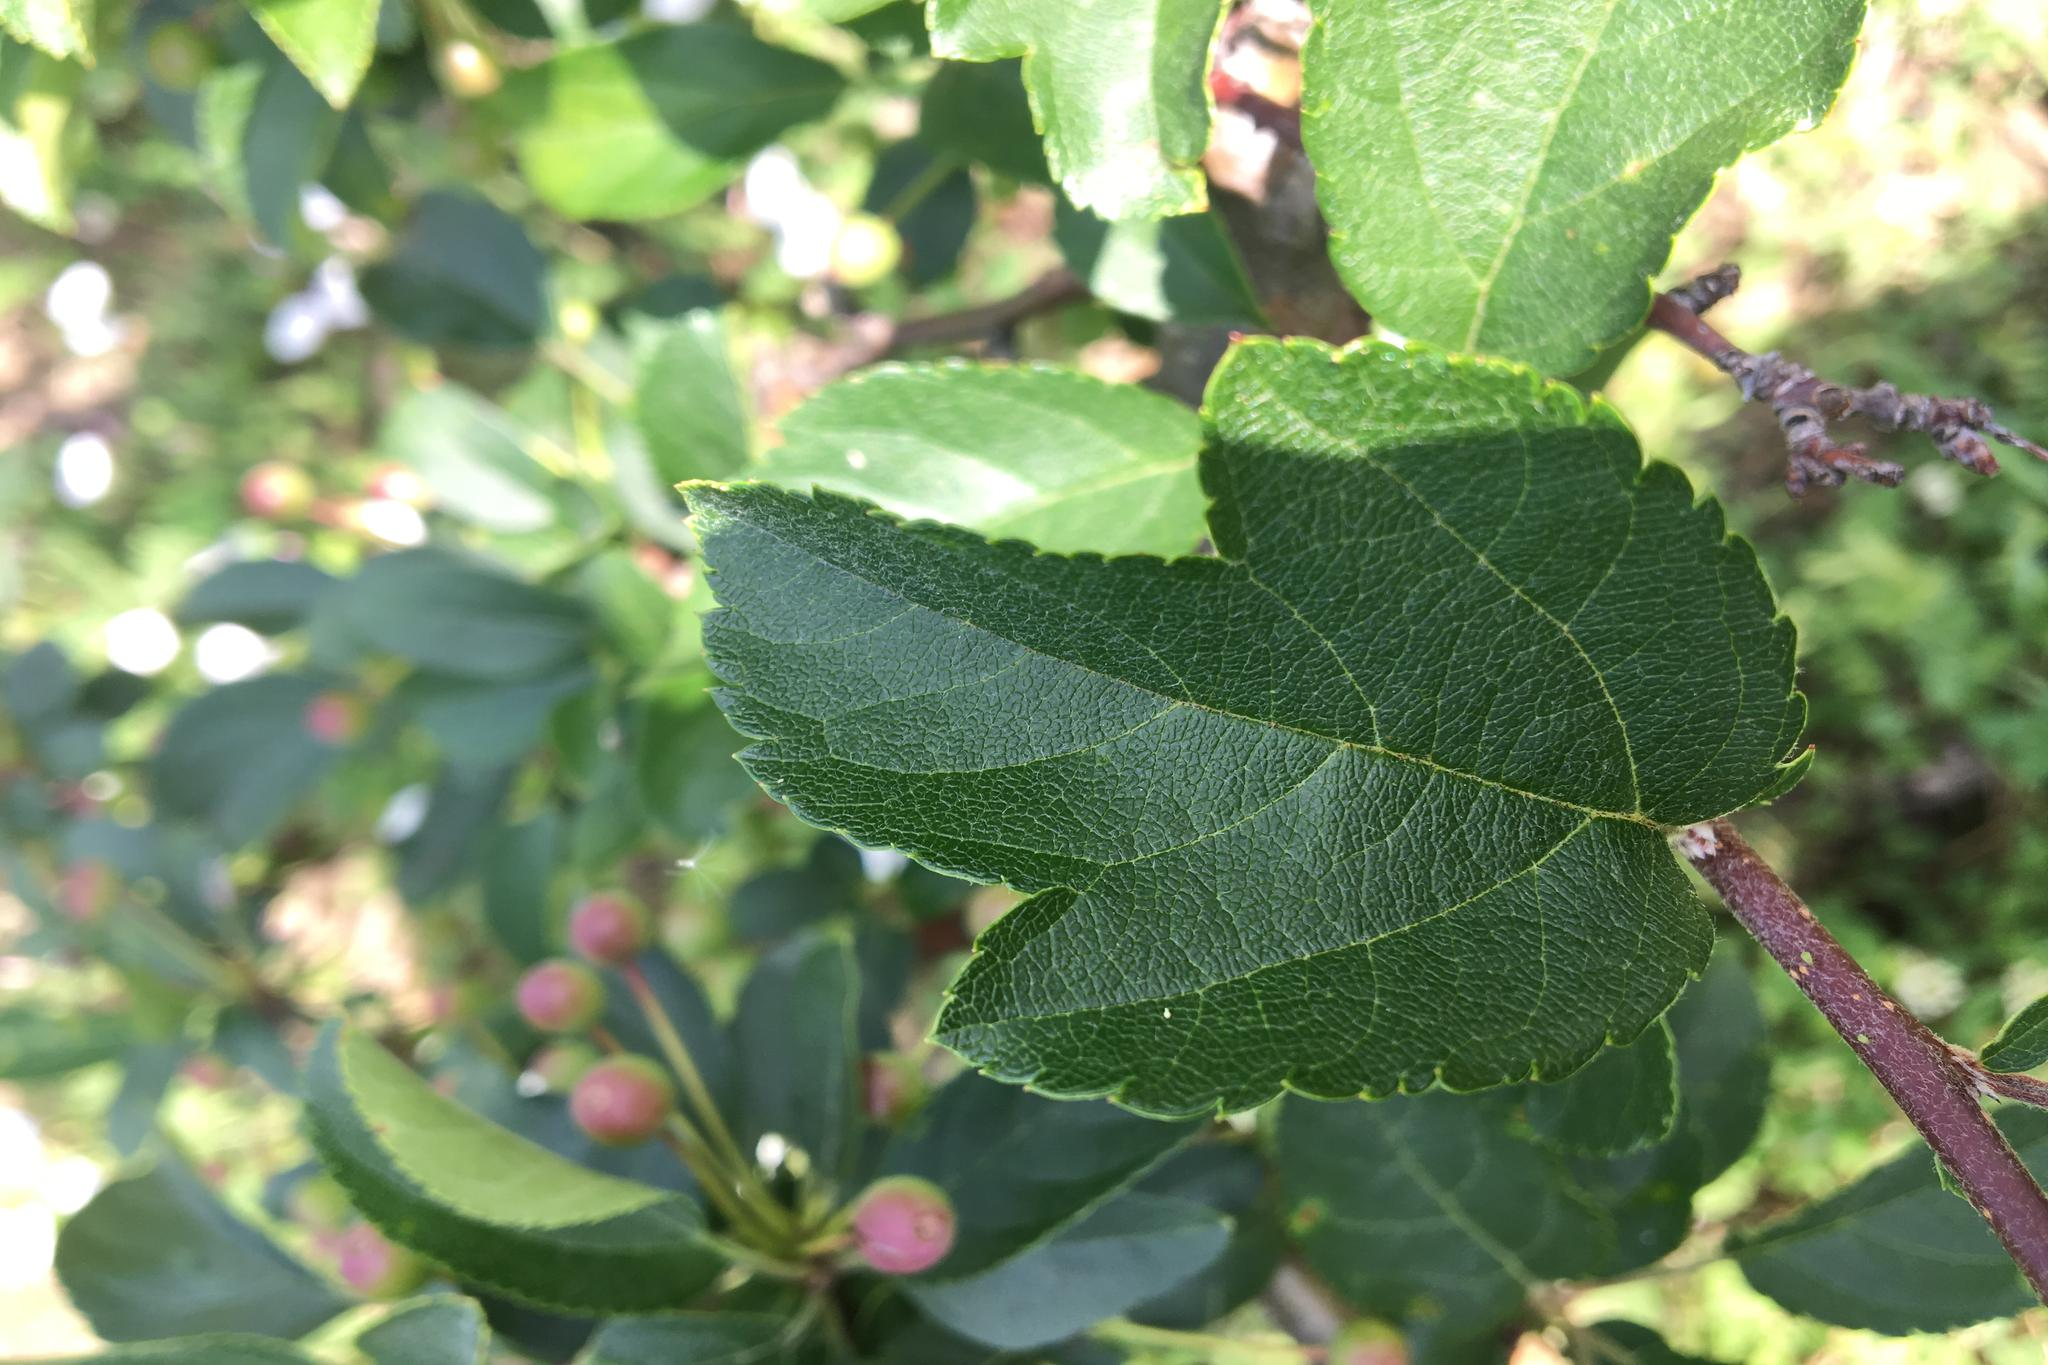
\includegraphics[width=.4\linewidth]{images/Test_1023.jpg}
  \caption{Original Image}
  \label{fig:sub1}
\end{subfigure}%
\begin{subfigure}{\textwidth}
  \centering
  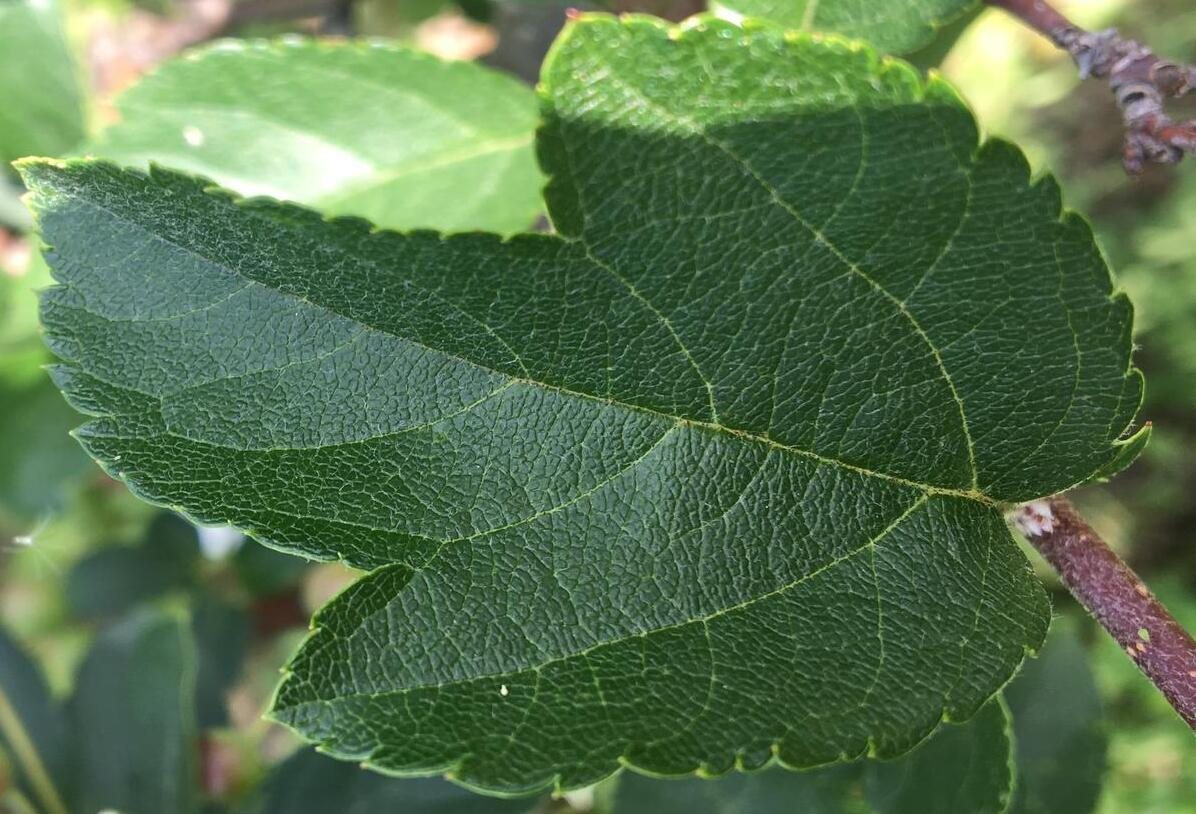
\includegraphics[width=.4\linewidth]{images/Test_1023_crpped.jpg}
  \caption{Image Cropped with canny edge detection}
  \label{fig:sub2}
\end{subfigure}
%\caption{Illustration of Flipping}
\label{fig:test}
\end{figure}

 
 
\end{itemize}
The result of these five steps is a two-dimensional binary map (0 or 255) indicating the location of edges on the image.

With this method we reduce the size of the image to focus only on the leaf. We cropped the Image as we can see on the following screen.






\begin{figure}[H]
      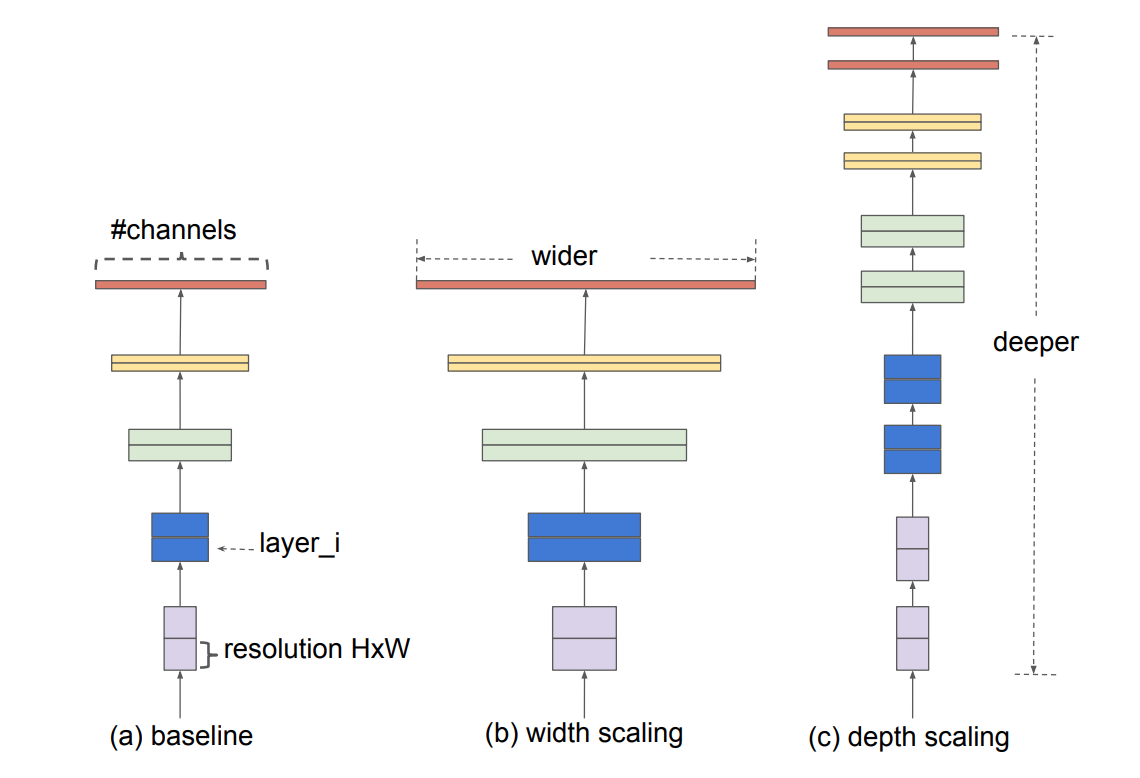
\includegraphics[width=\linewidth]{images/scaling.png}
      \caption{Illustration of scaling of DNNS : from \cite{DBLP:journals/corr/abs-1905-11946}}
      \label{fig:scaling}
\end{figure}


\subsection{Flipping : }

Flipping is a simple transformation that involves index switching on image channels. In vertical flipping, the order of the lines is exchanged. In vertical flipping, the order of the lines is exchanged. Let's assume that "long" and the "lag" is the size of the  
In order to perform the horizontal flipping the pixel (x, y) will be situated at coordinate (long - x + 1, y) in the new image.\\
\begin{itemize}
    \item {
    Horizontal Flip :  
    \begin{equation} 
	Horizontal Flip:  A_{ij} = A_{i(long +1 -j)}
	\end{equation}
	}
    \item{
    Vertical Flipping :
	\begin{equation} 
	Horizontal Flip:  A_{ij} = A_{(lag +1 -i)j}
	\end{equation}
    }

\end{itemize}

\begin{figure}[H]
\centering
\begin{subfigure}{\textwidth}
  \centering
  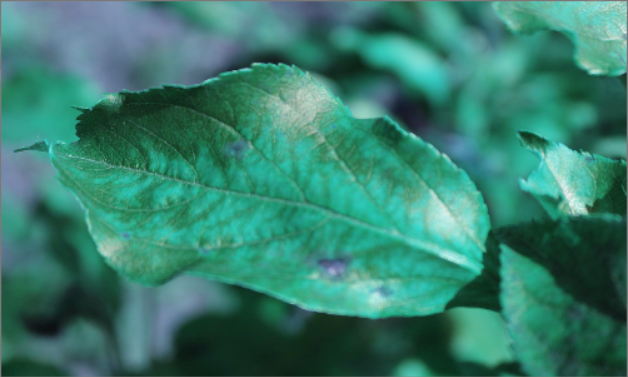
\includegraphics[width=.4\linewidth]{images/origina.png}
  \caption{Original Image}
  \label{fig:sub1}
\end{subfigure}%
\begin{subfigure}{\textwidth}
  \centering
  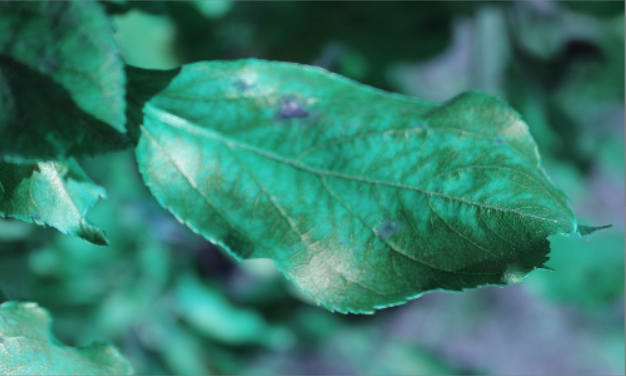
\includegraphics[width=.4\linewidth]{images/flipped.png}
  \caption{Image flipped}
  \label{fig:sub2}
\end{subfigure}
%\caption{Illustration of Flipping}
\label{fig:test}
\end{figure}


\subsection{Gaussian blur and Compression : } 
 As we know that sometimes the image quality taken for prediction can be a bad one,  we have to consider the quality of this image by making our model more robust. 
 Blurring is simply the addition of noise to the image, resulting in a less-clear image. The noise can be sampled from any distribution of choice, as long as the main content in the image does not become invisible. Only the minor details get obfuscated due to blurring.
 We can also use the image compression algorithms in order to decrease the image quality, in view to make the mode
 The following image is set to 90\% jpeg compression.
 
 \begin{figure}[H]
\centering
\begin{subfigure}{\textwidth}
  \centering
  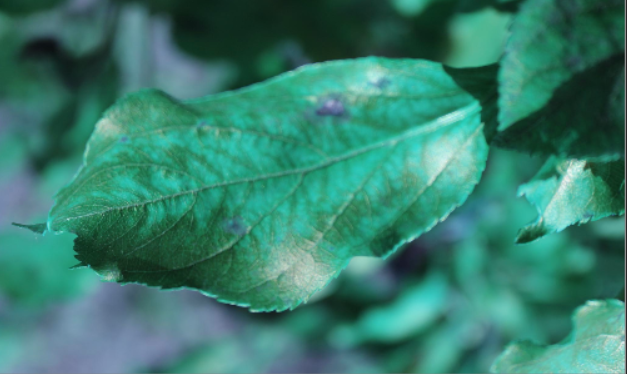
\includegraphics[width=.4\linewidth]{images/ori.png}
  \caption{Original Image}
  \label{fig:sub1}
\end{subfigure}%
\begin{subfigure}{\textwidth}
  \centering
  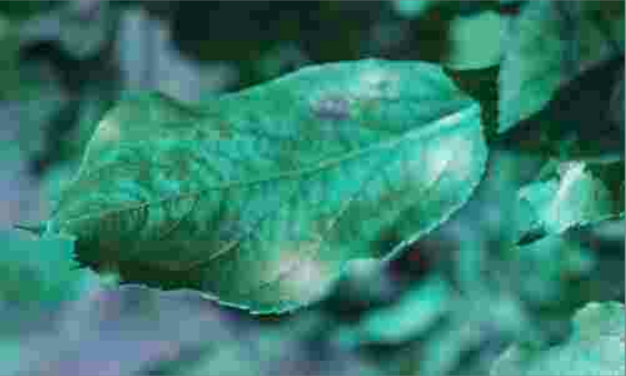
\includegraphics[width=.4\linewidth]{images/blur.png}
  \caption{Compressed Image}
  \label{fig:sub2}
\end{subfigure}
%\caption{Illustration of compression 10\%}
\label{fig:test}
\end{figure}

\subsection{Data Augmentation}
 
 
\section{Approaches of our model: }
In order to choose the most efficient model for our task of classification, we have decided to collect different benchmarks over recent papers which perform image classification in general and more precisely which perform plant pathology's detection tasks.
In view of the constraints of the domain due to the low power of the device which will host this model, we have to find the most efficient model which requires less memory space and computation power. 
To reach our goal, we read the following articles : \cite{canny}, \href{https://paperswithcode.com/task/image-classification}{link\ExternalLink}  \cite{stateOfArt}.  The website \href{https://paperswithcode.com/task/image-classification}{link \ExternalLink} presents in a synthetic way the benchmarks.
Through these papers and benchmarks, we keep on our notebook the following models: ResNet, and EfficientNet. Before diving deep into these models let's notice that in order to gain efficiency, we will train these models in transfer learning context.
Transfer Learning is the ability to reuse an trained model to solve other problems. The main purpose of Transfer learning is efficiency during training. It has been proven that training a model from scratch is more expensive than training a model from a pre-training model.
In our case, our model was pre-trained on  \href{http://www.image-net.org/}{ImageNet \ExternalLink}.
Let talk about the selected models :

\subsection{ResNet :}
ResNet stands for Residual network. This model appears in response to the gradient vanishing problem[10] in Convolution Neural Network with a large depth.
Let explain the context of apparition of this model. 
In the past to increase accuracy of image classification tasks, the basic approach was to scaling up the model. By adding more layers of convolution to the model or make greater the width of the network. The following schema ~\ref{fig:scaling} will explain different kinds of scaling up. 


    \begin{figure}[H]
      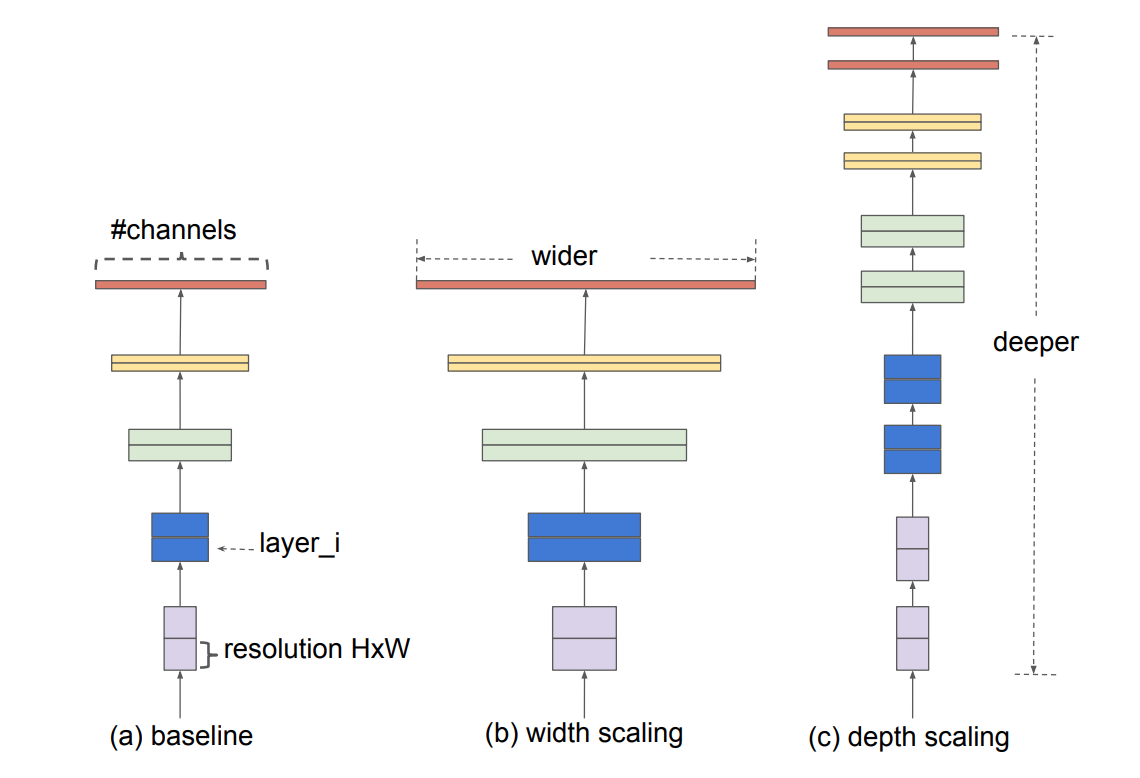
\includegraphics[width=\linewidth]{images/scaling.png}
      \caption{Illustration of scaling of DNNS : from \cite{DBLP:journals/corr/abs-1905-11946}}
      \label{fig:scaling}
    \end{figure}


But in this way, we need more and more power to compute the weights of this kind of network.
After a long time spent scaling up a single dimension at the same time(either channel, either width either depth) of the networks in order to improve the accuracy of classification, a main problem has been observed. 
This problem is the gradient vanishing problem \cite{vanishing}. As more layers using certain activation functions are added to neural networks, the gradients of the loss function approaches zero, making the network hard to train. Some activation functions, such as the sigmoid function, compress a large input space into a small input space between 0 and 1, so a large change in the sigmoid function input will result in a small change in the output. Consequently, the derivative becomes small.
For a shallow network with only a few layers using these activation's function, this is not a big problem. However, when multiple layers are used, the gradient can be too shallow for the training to perform well.
The gradients of the neural networks are determined using back-propagation. In very simple terms, back-propagation is used to find network derivatives by moving layer by layer from the top layer to the bottom layer. According to the chain rule, the derivatives of each layer are multiplied in the network (from the final layer to the initial layer) to calculate the derivatives of the initial layers.
However, when n hidden layers use an activation like the sigmoid function, n small derivatives are multiplied together. Thus, the gradient decreases exponentially as we propagate down to the initial layers.
A small gradient means that the weights and biases of the initial layers will not be updated effectively with each training. As these initial layers are often crucial in recognising the essential elements of the input data, this can lead to an overall inaccuracy of the entire network.



\begin{itemize}
    \item{The simplest solution is to use other activation functions, such as ReLU, which does not cause a small derivative.}
    \item{Also, batch normalization layers can fix the issue. The problem is occurred when a large range of input is mapped to a tiny one. Batch normalization reduces this problem by normalizing the input.}
    \item{Another solution is the Residual network. It is characterized by the residual connections straight to earlier layers. The residual connection directly adds the value at the beginning of the block, to the end of the block (F(x)+x). This residual link does not go through activation functions that "overwrite" the derivatives, resulting in a higher overall derivative of the block.
    }
\end{itemize}
In view of these problems, we saw the creation of a new network called Residual neural network ( ResNet ) . The following figure ~\ref{fig:resnet} sums up the new approach :

 \begin{figure}[H]
      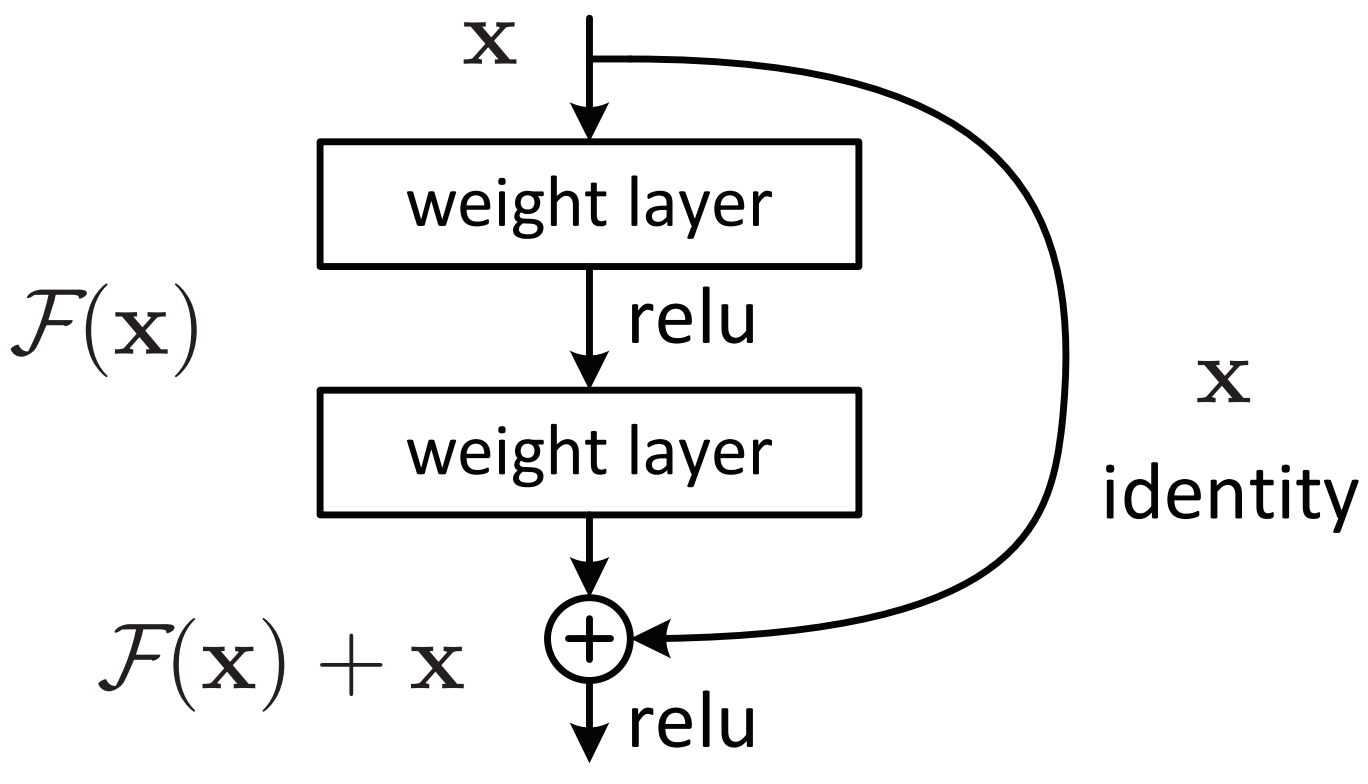
\includegraphics[width=\linewidth]{images/resnet.png}
      \caption{Resnet Minimum architecture:from \cite{he2015deep}}
      \label{fig:resnet}
    \end{figure}

The main idea of the ResNet is from Cortex visual of the Human. In fact they added the highway to the architecture. This highway (having the identity function on the input) will “amplify” the output change according to the input change.
In the ResNet context of scaling up CNNs, many variants have been created. 
To scale up the ResNet architecture we have to add more layers. For instance  From ResNet-18 to ResNet-200, we add more layers. The obtained network will be more accurate if we can train it. 
Now let’s explain our own resnet model.  We use \textbf{ResNet-50}. As mentioned in his name it uses 50 layers.
Now that our ResNet model has \textbf{23,858,500} parameters, \textbf{23,805,380} Trainable parameters and non-trainable parameters: 53,120. On the top of this ResNet-50 we add one layer of GlobalAveragePooling2D, another of 128 neurons with relu function for activation, another one of 64 neurons with relu activation and the last one with 4 neurons with softmax activation to get the output like a probability.
The optimizer which we have used is the Adam optimizer. 
The results that we got will be presented in the result section of the document.


\subsection{EfficientNet :}

Once the gradient vanishing problem was solved with the ResNet architecture, we noticed that there is no formal way to scale up the network. In fact there is no formal way to choose which dimension (width, depth or Resolution) scales in which distribution in order to increase the accuracy and minimize the cost (computational cost, memory cost).
Although we succeeded in training these models, we can see that the accuracy will be saturated after a certain level of scaling. As shown in the following figure ~\ref{fig:scaling_multi}. 

    \begin{figure}[H]
      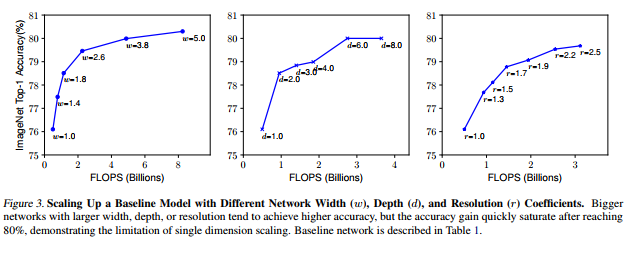
\includegraphics[width=\linewidth]{images/scaling_one.png}
      \caption{Accuracy over scaling on one dimension:from \cite{DBLP:journals/corr/abs-1905-11946}}
      \label{fig:scaling_multi}
    \end{figure}

Let’s notice that with w = 5.0 (scaling on one dimension width) they got the saturation of accuracy. With d=8.0 (scaling on one dimension width) we also get the saturation of accuracy and with r=2.5  we get the saturation of accuracy. 
But the researchers noticed that in the following schema with depth= 2.0 and r=1.3 the saturation event didn't occurred. 

    \begin{figure}[H]
      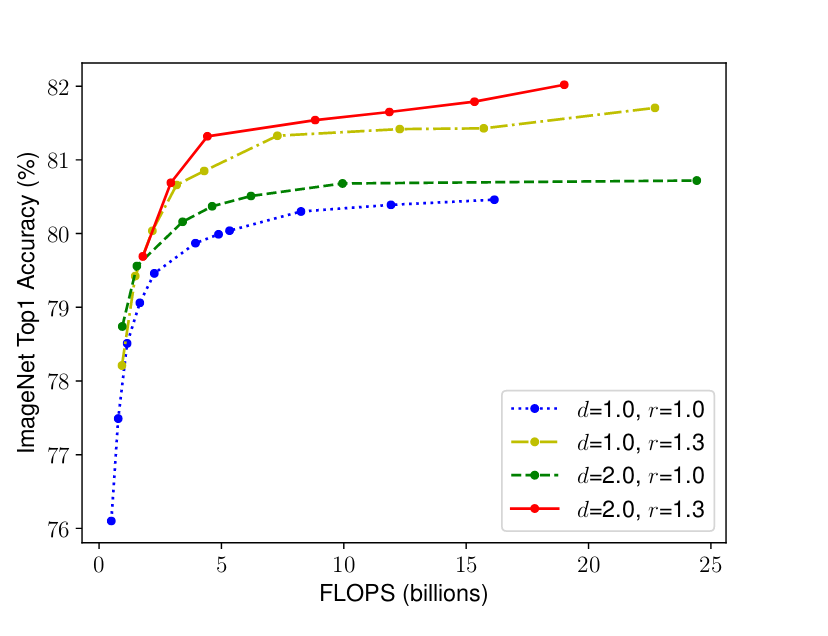
\includegraphics[width=\linewidth]{images/efficeint.png}
      \caption{Impact on accuracy over scaling on multiple dimensions:from \cite{DBLP:journals/corr/abs-1905-11946}}
      \label{fig:scaling_multi}
    \end{figure}
    
Each dot is a model with different width. Where here, they conclude that the right solution can be scaling up the network on multiple dimensions (depth and resolution).
The previous problems or situations caused the creation of the new approach or technique of scaling up the network on multiple dimensions. 
This technique (model) rethinks the way that we scale CNNs up. In addition, this new technique has posed certain constraints to be satisfied. 
\begin{itemize}
    \item {maximize the model accuracy for any given resource constraints. }
    \item { To systematically study model scaling and balance the network depth, width and resolution.}
\end{itemize}

In more formal way : with the model N, the objective function will be
       \begin{figure}[H]
      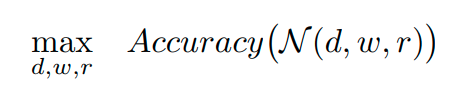
\includegraphics[scale=0.25]{images/accurat.png}
      \caption{Objective function :from \cite{DBLP:journals/corr/abs-1905-11946}}
      \label{fig:scaling_multi}
    \end{figure}
    
With the following constraints: 

       \begin{figure}[H]
        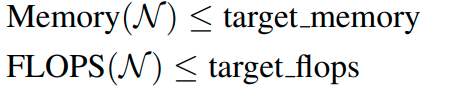
\includegraphics[scale=0.25]{images/condition.png}
            \caption{Constraints of equations: from \cite{DBLP:journals/corr/abs-1905-11946}}
        \label{fig:scaling_multi}
        \end{figure}
     
        
To solve this problem EfficientNet proposes the \textbf{Compound scaling method}. This scaling method tries to balance dimensions of width/depth/resolution by scaling with a constant ratio.
Let’s notice that this new approach uses an existing architecture and propose a way to efficiently scale up this one with a Compound scaling method.
This new approach states that : 
\\
  
       $2^n$ more computational resources implies $a^n$ + $b^n$ + $c^2$ additional dimensions on the model.


The coefficient a, b and c are constants determined by a small GRID SEARCH on the original small model.
Let's notice that $a^n$ is the additional value to the depth dimension of the model , $b^n$ is the additional value to the width dimension of the model and $c^n$ is the additional value to the  resolution dimension of the model.
The following equation allows to get the different coefficients :
	\begin{equation} 
            a + b^2 + c^2 \approx 2
	\end{equation}

from the original paper that is formulated as following : 
Thanks to this new way, the researchers realized the best accuracy with less parameters (less resources). As we can show on the following figure ~\ref{fig:perf} from original paper.
       
        \begin{figure}[H]
        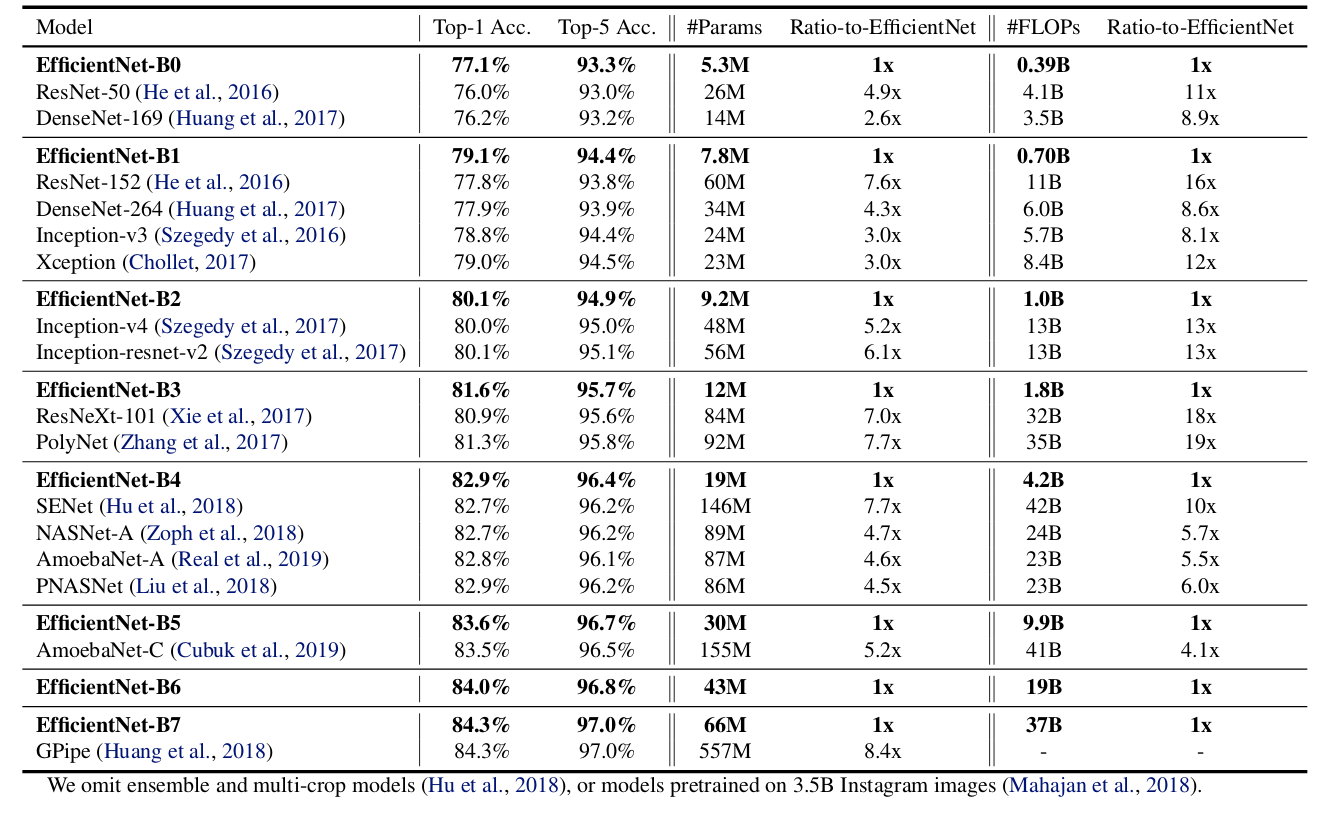
\includegraphics[width=\linewidth]{images/perf.png}
            \caption{Gain of performance on different models: from \cite{DBLP:journals/corr/abs-1905-11946}}
        \label{fig:perf}
        \end{figure}
        
We can show on the first row, with EfficientNet-B0 there are 5.3M parameters and they got as accuracy 77.1\% and with ResNet-50 there are 26M and they got as accuracy 76.0 \%. The gain of the performance here is awesome.
    
We have used EfficientNetB7 adding GlobalAveragePooling layer, 3 Dense layer as following :
\begin{itemize}
    \item {dense3 (Dense): with the following shape (None, 128) and parameters 327808}
    \item {dense4 (Dense): with the following shape (None, 64) and parameters 8256}
    \item {dense5 (Dense): with the following shape (None, 4) and parameters 260}
\end{itemize}

We coupled this model with Self-Training Noisy student \cite{xie2020selftraining}. This technique allows us to improve the accuracy of the model.


\section{Result and Interpretation:}
\subsection{Result}
In this section we will present the result of our study. We start with accuracy and Epochs plot in order to show how the accuracy will increase over the time.




   \begin{figure}[H]
        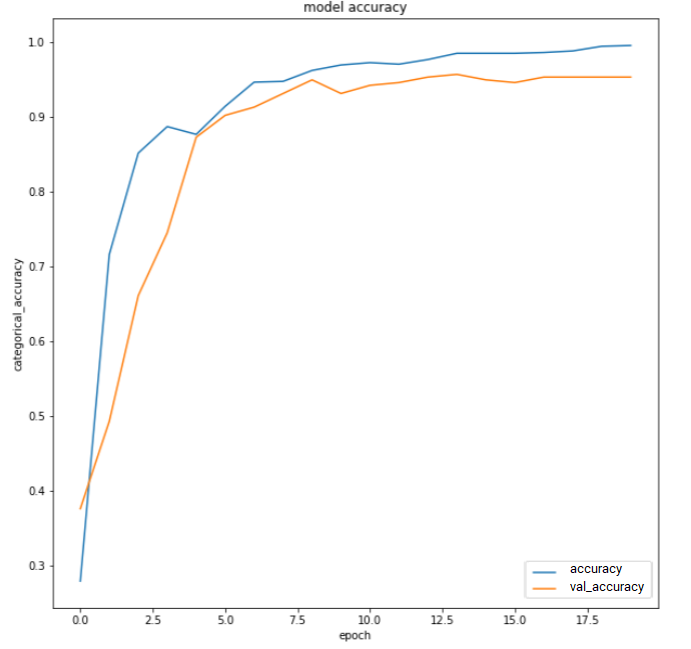
\includegraphics[width=\linewidth]{images/new_one.png}
            \caption{Dense Accuracy Plot over epochs}
        \label{fig:dense_accu}
        \end{figure}    
This plot ~\ref{fig:dense_accu} shows the convergence of the average. We got 0.97 as accuracy on the training set and the 0.93 on the test set. With this last one we can see easily that the model works well on the training than the training set. Obviously this is normal. Our DenseNet is a standard CNNs.

  \begin{figure}[H]
    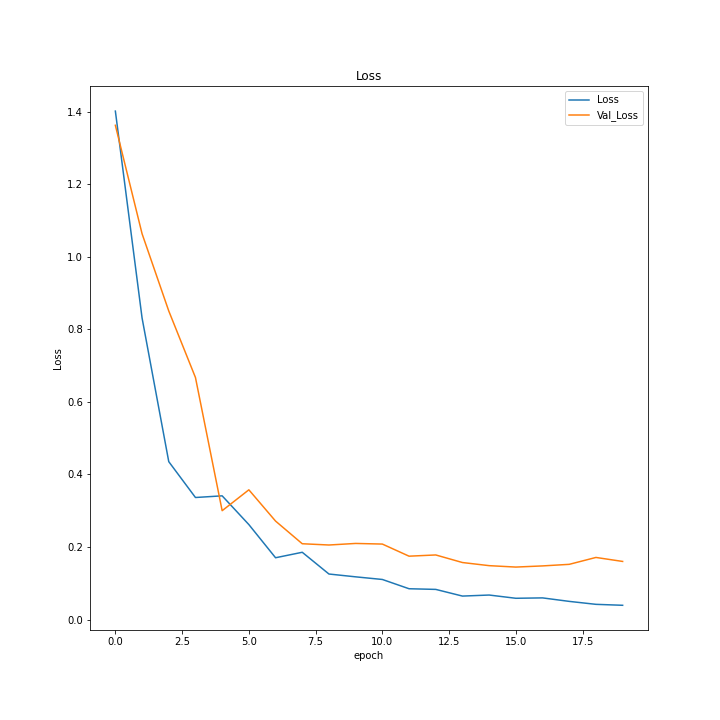
\includegraphics[width=\linewidth]{images/history22_loss.png}
            \caption{Dense Loss Plot over epochs}
    \label{fig:loss_dense}
  \end{figure}    
This plot  ~\ref{fig:loss_dense} shows the evolution of the loss value over the time. Obviously the loss converges to 0 over contrary the accuracy.

 \begin{figure}[H]
    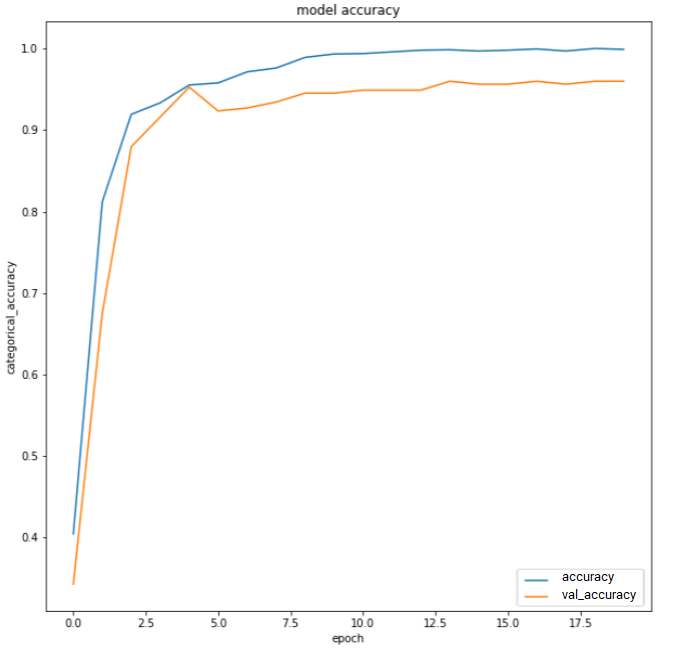
\includegraphics[width=\linewidth]{images/new_2.png}
            \caption{Dense Accurate with filter Plot over epochs}
    \label{fig:desne_filter_accu}
  \end{figure} 
 
 In this Network we add more filter in image in order to decrease the quality of this ones and we train our dense with them. This manipulation is done in order to make the model more robust. The figure ~\ref{fig:desne_filter_accu}
 shows the accuracy gotten.
 \begin{figure}[H]
    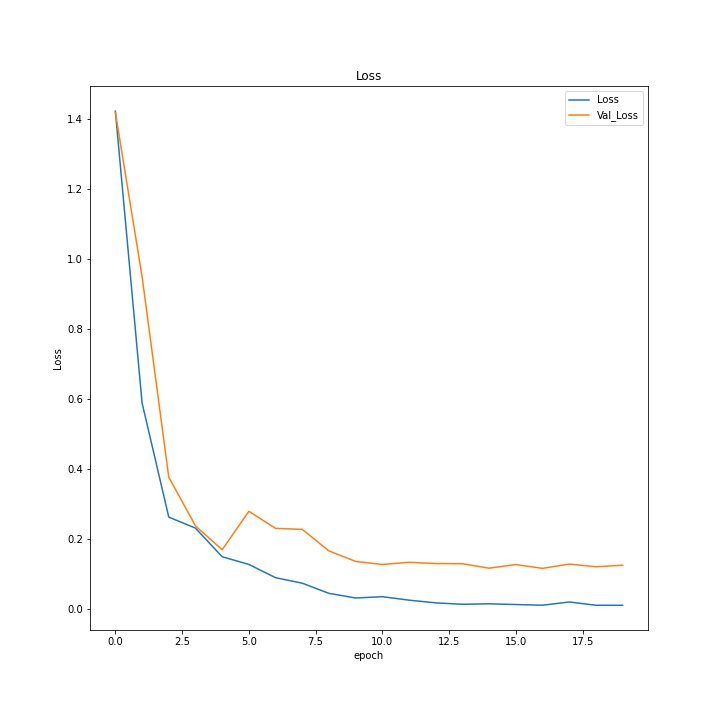
\includegraphics[width=\linewidth]{images/history222_loss.png}
            \caption{Dense Loss with filter Plot over epochs}
    \label{fig:desne_filter_loss}
  \end{figure}  
  This is the plot ~\ref{fig:desne_filter_loss} distribution over the epochs with the filter applied in the DenseNEt 
\begin{figure}[H]
    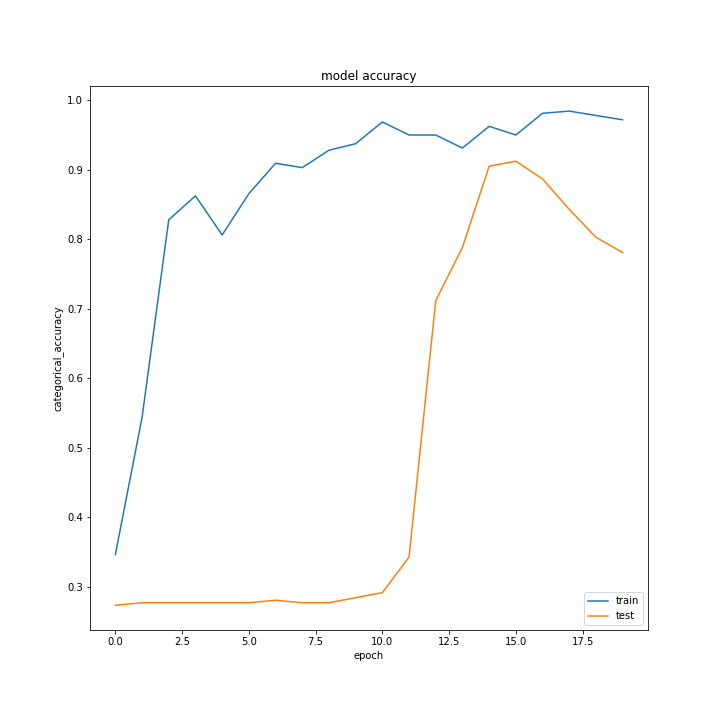
\includegraphics[width=\linewidth]{images/resnet_accu.png}
            \caption{Resnet Accuracy with filter Plot over epochs}
    \label{fig:resnet_accu}
  \end{figure}  
This plot ~\ref{fig:resnet_accu} shows the distribution of the accuracy of the epoch with res-net. Obviously we can notice this network make a lot of time before to converge in a test set. This is due to the effect of the filter on the training set and also we didn't apply these filters on the test set. 


 \begin{figure}[H]
    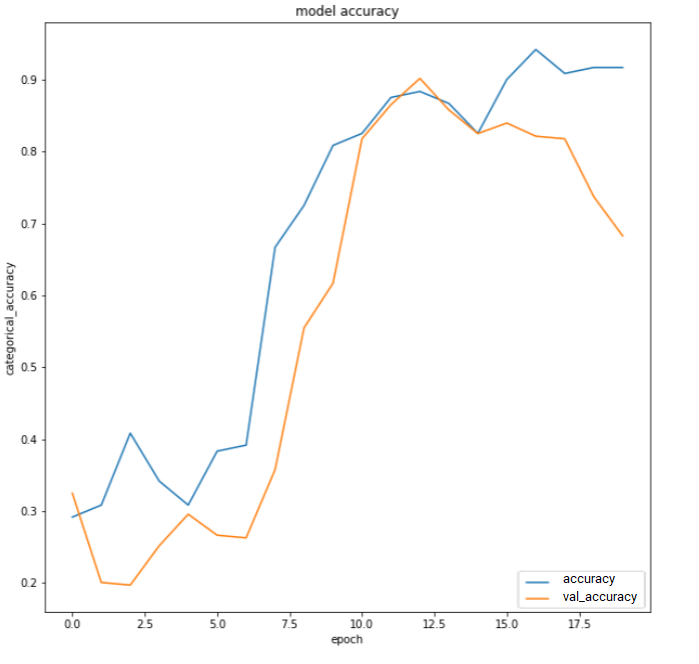
\includegraphics[width=\linewidth]{images/new_eff.png}
            \caption{EfficientNet Accuracy with filter Plot over epochs}
    \label{fig:effiaccu}
 \end{figure}
 This plot ~\ref{fig:effiaccu} shows the performance of the EfficientNet on this Dataset. As specified previously, we have used EfficienNet-B7. We got a couple of the issues due the size of this network. We fixed it, and we got as the accuracy 0.91 on the training set and 0.7 on the test set. We stop training because we got the stack-overflow on Server.
 But fro, kaggle and others resources; EfficientNet is the suitable network for this task.
 \begin{figure}[H]
    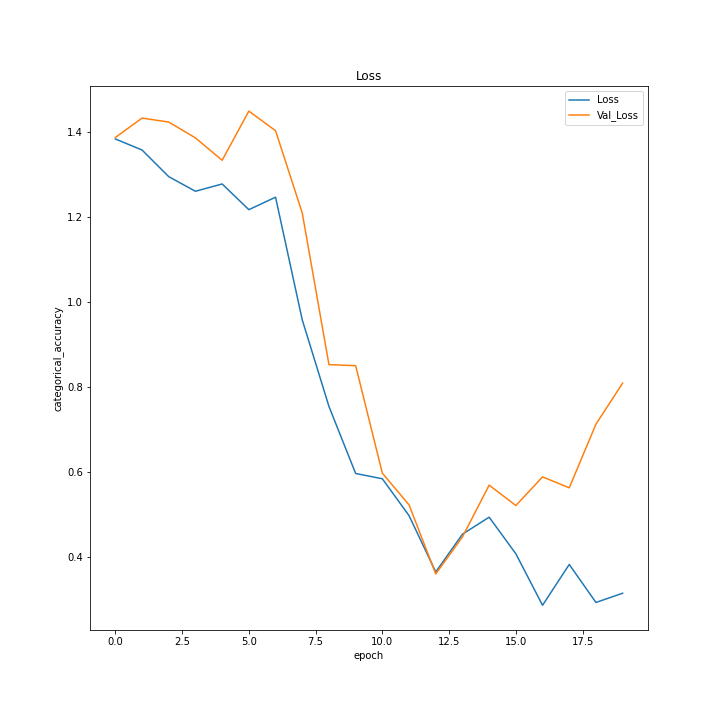
\includegraphics[width=\linewidth]{images/eff_loss.png}
            \caption{EfficientNet Loss with filter Plot over epochs}
    \label{fig:histoty_dense}
  \end{figure}    

This plot represents the loss distribution of the EfficientNet-B7 on our dataset
  
 \begin{figure}[H]
    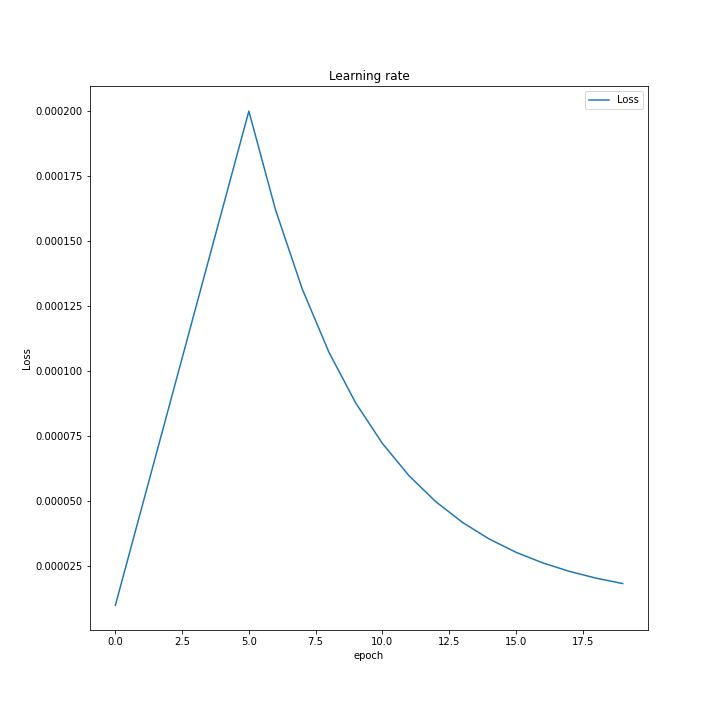
\includegraphics[width=\linewidth]{images/history_lr.png}
            \caption{Learning rate distribution over epochs}
    \label{fig:histoty_dense}
  \end{figure}    
 
  
  
\subsection{Interpretation : }

Form different papers on the Plant pathology detection with Deep Learning we browsed, the most efficient model was the EfficientNet. But after long time on the subject with this dataset, we can say that DenseNet (simple CNN) is more suitable for this specify dataset than the others. 
From This result, we can interpret that our dataset is not enough large, and our server test is not powerful enough to train the Resnet and EfficientNet to beat the single DenseNet. 

\newpage
\listoffigures
\newpage
\bibliographystyle{IEEEtran}
\bibliography{sample}


\end{document}